% Options for packages loaded elsewhere
\PassOptionsToPackage{unicode}{hyperref}
\PassOptionsToPackage{hyphens}{url}
%
\documentclass[
  ignorenonframetext,
  aspectratio=169,
  russian,
]{beamer}
\usepackage{pgfpages}
\setbeamertemplate{caption}[numbered]
\setbeamertemplate{caption label separator}{: }
\setbeamercolor{caption name}{fg=normal text.fg}
\beamertemplatenavigationsymbolshorizontal
% Prevent slide breaks in the middle of a paragraph
\widowpenalties 1 10000
\raggedbottom
\setbeamertemplate{part page}{
  \centering
  \begin{beamercolorbox}[sep=16pt,center]{part title}
    \usebeamerfont{part title}\insertpart\par
  \end{beamercolorbox}
}
\setbeamertemplate{section page}{
  \centering
  \begin{beamercolorbox}[sep=12pt,center]{section title}
    \usebeamerfont{section title}\insertsection\par
  \end{beamercolorbox}
}
\setbeamertemplate{subsection page}{
  \centering
  \begin{beamercolorbox}[sep=8pt,center]{subsection title}
    \usebeamerfont{subsection title}\insertsubsection\par
  \end{beamercolorbox}
}
\AtBeginPart{
  \frame{\partpage}
}
\AtBeginSection{
  \ifbibliography
  \else
    \frame{\sectionpage}
  \fi
}
\AtBeginSubsection{
  \frame{\subsectionpage}
}

\usepackage{amsmath,amssymb}
\usepackage{iftex}
\ifPDFTeX
  \usepackage[T1]{fontenc}
  \usepackage[utf8]{inputenc}
  \usepackage{textcomp} % provide euro and other symbols
\else % if luatex or xetex
  \usepackage{unicode-math}
  \defaultfontfeatures{Scale=MatchLowercase}
  \defaultfontfeatures[\rmfamily]{Ligatures=TeX,Scale=1}
\fi
\usepackage{lmodern}
\usetheme[]{Madrid}
\usecolortheme{default}
\usefonttheme{professionalfonts}
\ifPDFTeX\else  
    % xetex/luatex font selection
\fi
% Use upquote if available, for straight quotes in verbatim environments
\IfFileExists{upquote.sty}{\usepackage{upquote}}{}
\IfFileExists{microtype.sty}{% use microtype if available
  \usepackage[]{microtype}
  \UseMicrotypeSet[protrusion]{basicmath} % disable protrusion for tt fonts
}{}
\usepackage{xcolor}
\newif\ifbibliography
\setlength{\emergencystretch}{3em} % prevent overfull lines
\setcounter{secnumdepth}{-\maxdimen} % remove section numbering


\providecommand{\tightlist}{%
  \setlength{\itemsep}{0pt}\setlength{\parskip}{0pt}}\usepackage{longtable,booktabs,array}
\usepackage{calc} % for calculating minipage widths
\usepackage{caption}
% Make caption package work with longtable
\makeatletter
\def\fnum@table{\tablename~\thetable}
\makeatother
\usepackage{graphicx}
\makeatletter
\newsavebox\pandoc@box
\newcommand*\pandocbounded[1]{% scales image to fit in text height/width
  \sbox\pandoc@box{#1}%
  \Gscale@div\@tempa{\textheight}{\dimexpr\ht\pandoc@box+\dp\pandoc@box\relax}%
  \Gscale@div\@tempb{\linewidth}{\wd\pandoc@box}%
  \ifdim\@tempb\p@<\@tempa\p@\let\@tempa\@tempb\fi% select the smaller of both
  \ifdim\@tempa\p@<\p@\scalebox{\@tempa}{\usebox\pandoc@box}%
  \else\usebox{\pandoc@box}%
  \fi%
}
% Set default figure placement to htbp
\def\fps@figure{htbp}
\makeatother

\IfFileExists{plex-otf.sty}{
  %% Full TeXlive
  % \usepackage[%
  %   % math,
  %   RM={Scale=0.94},SS={Scale=0.94},SScon={Scale=0.94},TT={Scale=MatchLowercase,FakeStretch=0.9},DefaultFeatures={Ligatures=Common}
  % ]{plex-otf}
}{
  %% TinyTeX
  \usepackage{libertine}
}

%%% Load theme
% https://deic.uab.cat/~iblanes/beamer_gallery/
\IfFileExists{beamerthemegotham.sty}{
  %% Full TeXlive
  \usetheme{gotham}
  \gothamset{
    numbering=totalpagenumber,
    parttocframe default=off,
    sectiontocframe default=off,
    subsectiontocframe default=off,
  }
}{
  %% TinyTeX
  \usetheme{Madrid}
}
\metroset{progressbar=frametitle,sectionpage=progressbar,numbering=fraction}
\makeatletter
\beamer@ignorenonframefalse
\makeatother
\makeatletter
\@ifpackageloaded{caption}{}{\usepackage{caption}}
\AtBeginDocument{%
\ifdefined\contentsname
  \renewcommand*\contentsname{Содержание}
\else
  \newcommand\contentsname{Содержание}
\fi
\ifdefined\listfigurename
  \renewcommand*\listfigurename{Список иллюстраций}
\else
  \newcommand\listfigurename{Список иллюстраций}
\fi
\ifdefined\listtablename
  \renewcommand*\listtablename{Список таблиц}
\else
  \newcommand\listtablename{Список таблиц}
\fi
\ifdefined\figurename
  \renewcommand*\figurename{Рисунок}
\else
  \newcommand\figurename{Рисунок}
\fi
\ifdefined\tablename
  \renewcommand*\tablename{Таблица}
\else
  \newcommand\tablename{Таблица}
\fi
}
\@ifpackageloaded{float}{}{\usepackage{float}}
\floatstyle{ruled}
\@ifundefined{c@chapter}{\newfloat{codelisting}{h}{lop}}{\newfloat{codelisting}{h}{lop}[chapter]}
\floatname{codelisting}{Список}
\newcommand*\listoflistings{\listof{codelisting}{Листинги}}
\makeatother
\makeatletter
\makeatother
\makeatletter
\@ifpackageloaded{caption}{}{\usepackage{caption}}
\@ifpackageloaded{subcaption}{}{\usepackage{subcaption}}
\makeatother

\ifLuaTeX
\usepackage[bidi=basic]{babel}
\else
\usepackage[bidi=default]{babel}
\fi
\babelprovide[main,import]{russian}
\babelprovide[import]{english}
% get rid of language-specific shorthands (see #6817):
\let\LanguageShortHands\languageshorthands
\def\languageshorthands#1{}
\usepackage{csquotes}
\usepackage{bookmark}

\IfFileExists{xurl.sty}{\usepackage{xurl}}{} % add URL line breaks if available
\urlstyle{same} % disable monospaced font for URLs
\hypersetup{
  pdftitle={Отчёт по выполнению лабораторной работы №1},
  pdfauthor={Пашутина Анна Алексеевна},
  pdflang={ru-RU},
  hidelinks,
  pdfcreator={LaTeX via pandoc}}


\title{Отчёт по выполнению лабораторной работы №1}
\subtitle{Установка и настройка Fedora Sway}
\author{Пашутина Анна Алексеевна}
\date{Invalid Date}
\institute{Российский университет дружбы народов, Москва, Россия}

\begin{document}
\frame{\titlepage}


\section{Информация}\label{ux438ux43dux444ux43eux440ux43cux430ux446ux438ux44f}

\begin{frame}{Докладчик}
\phantomsection\label{ux434ux43eux43aux43bux430ux434ux447ux438ux43a}
\begin{columns}[c]
\begin{column}{0.7\linewidth}
\begin{itemize}[<+->]
\tightlist
\item
  Пашутина Анна Алексеевна
\item
  Студентка
\item
  Российский университет дружбы народов
\item
  1032253642@pfur.ru
\end{itemize}
\end{column}

\begin{column}{0.3\linewidth}
\end{column}
\end{columns}
\end{frame}

\begin{frame}{Цель}
\phantomsection\label{ux446ux435ux43bux44c}
Целью данной работы является приобретение практических навыков установки
операционной системы на виртуальную машину, настройки минимально
необходимых для дальнейшей работы сервисов.
\end{frame}

\section{Задание}\label{ux437ux430ux434ux430ux43dux438ux435}

\begin{frame}{Задание}
\begin{itemize}[<+->]
\tightlist
\item
  Установка операционной системы
\item
  Установка драйверов для VirtualBox
\item
  Настройка раскладки клавиатуры
\item
  Установка имени пользователя и названия хоста
\item
  Подключение общей папки
\item
  Установка программного обеспечения для создания документации
\item
  Домашнее задание
\end{itemize}
\end{frame}

\begin{frame}{Установка Fedora Sway}
\phantomsection\label{ux443ux441ux442ux430ux43dux43eux432ux43aux430-fedora-sway}
Для начала создадим виртуальную машину. Укажем имя ВМ и адрес к
загрузочному носителю.

\begin{figure}[H]

{\centering 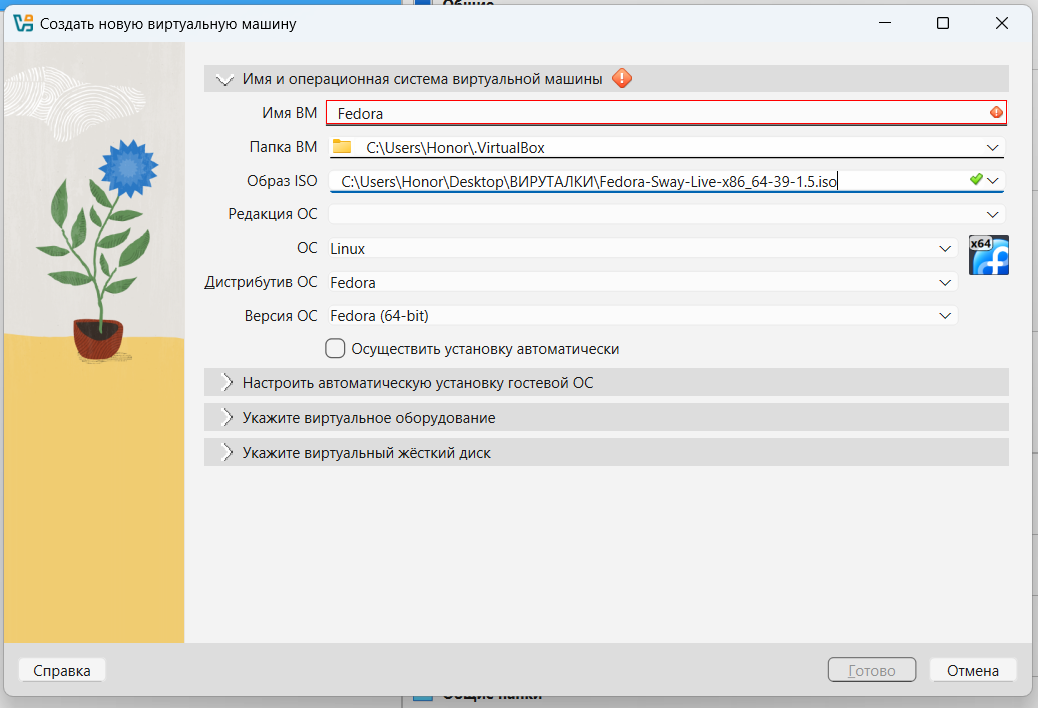
\includegraphics[width=\linewidth,height=0.66\textheight,keepaspectratio]{image/image1.png}

}

\caption{Указание имени ВМ и адреса к загрузочному носителю}

\end{figure}%
\end{frame}

\begin{frame}{Установка Fedora Sway}
\phantomsection\label{ux443ux441ux442ux430ux43dux43eux432ux43aux430-fedora-sway-1}
Далее выделим основную память.

\begin{figure}[H]

{\centering 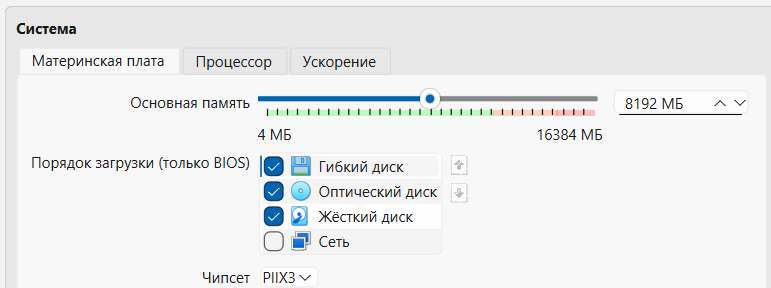
\includegraphics[width=\linewidth,height=0.66\textheight,keepaspectratio]{image/image2.png}

}

\caption{Выделение основной памяти для ВМ}

\end{figure}%
\end{frame}

\begin{frame}{Установка Fedora Sway}
\phantomsection\label{ux443ux441ux442ux430ux43dux43eux432ux43aux430-fedora-sway-2}
Далее выделим число ЦПУ и предел нагрузки для ВМ.

\begin{figure}[H]

{\centering 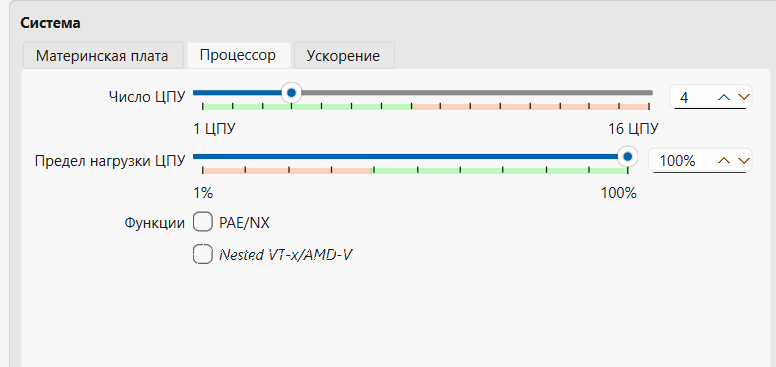
\includegraphics[width=\linewidth,height=0.66\textheight,keepaspectratio]{image/image3.png}

}

\caption{Выделение числа ЦПУ и предела нагрузки для ВМ}

\end{figure}%
\end{frame}

\begin{frame}{Установка Fedora Sway}
\phantomsection\label{ux443ux441ux442ux430ux43dux43eux432ux43aux430-fedora-sway-3}
Выделим виртуальный диск размером в 80 ГБ.

\begin{figure}[H]

{\centering 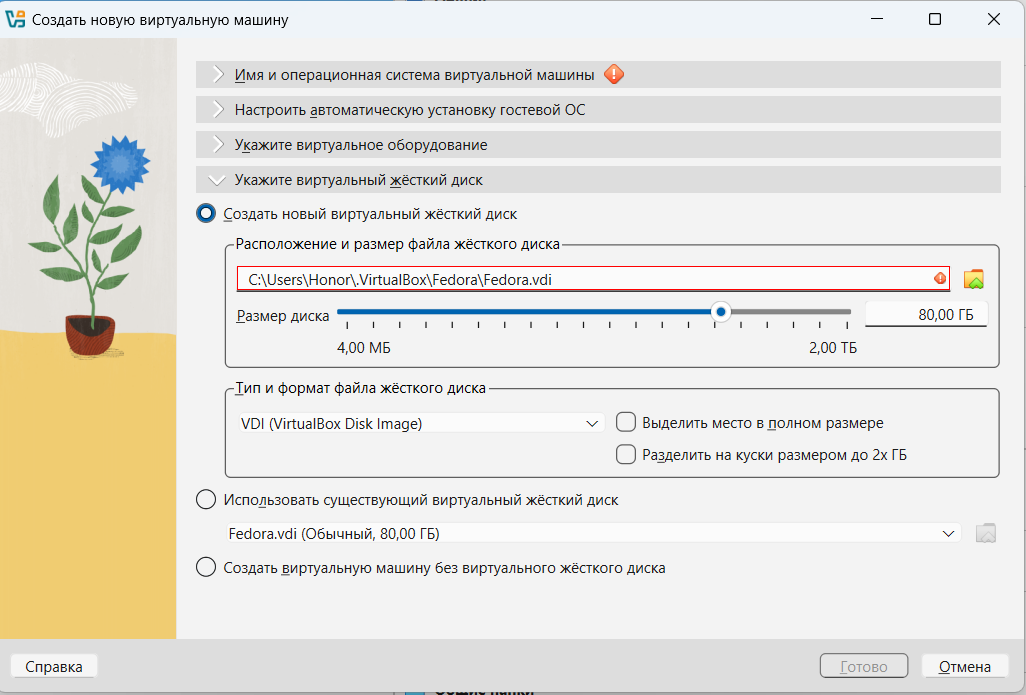
\includegraphics[width=\linewidth,height=0.66\textheight,keepaspectratio]{image/image4.png}

}

\caption{Выделение виртуального диска размером 80 ГБ}

\end{figure}%
\end{frame}

\begin{frame}{Установка Fedora Sway}
\phantomsection\label{ux443ux441ux442ux430ux43dux43eux432ux43aux430-fedora-sway-4}
Далее выделим видеопамять в 128 МБ и включим 3D ускорение.

\begin{figure}[H]

{\centering 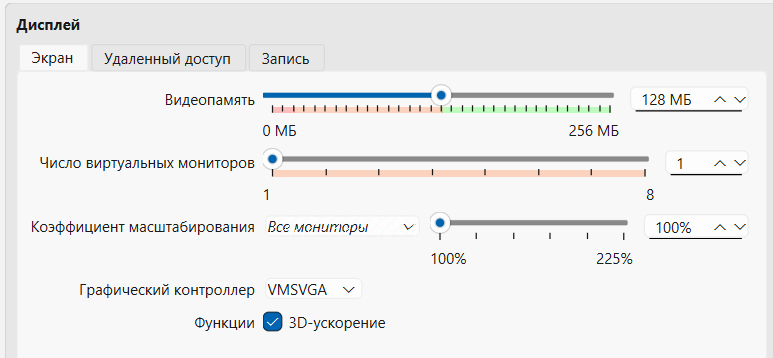
\includegraphics[width=\linewidth,height=0.66\textheight,keepaspectratio]{image/image5.png}

}

\caption{Выделение видеопамяти и включение 3D ускорения}

\end{figure}%
\end{frame}

\begin{frame}{Установка Fedora Sway}
\phantomsection\label{ux443ux441ux442ux430ux43dux43eux432ux43aux430-fedora-sway-5}
Запустим ВМ и запустим установщик Liveinst.

\begin{figure}[H]

{\centering 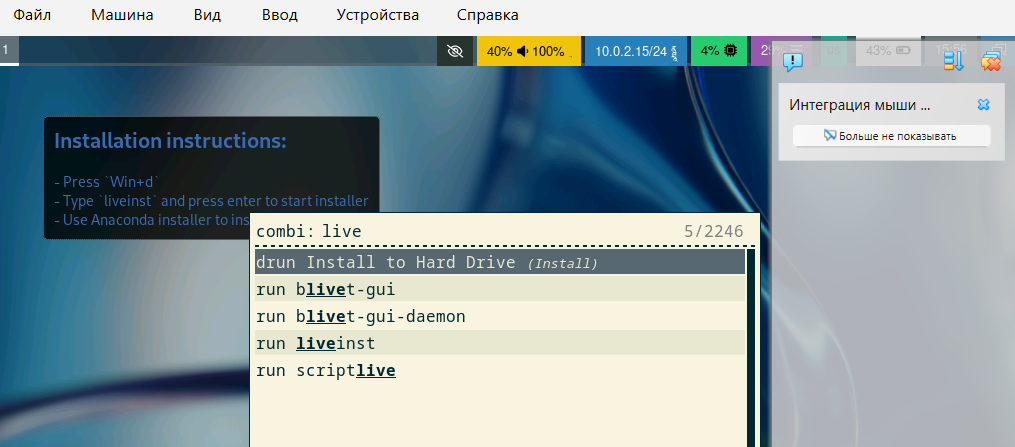
\includegraphics[width=\linewidth,height=0.66\textheight,keepaspectratio]{image/image6.png}

}

\caption{Запуск ВМ и установщика Liveinst}

\end{figure}%
\end{frame}

\begin{frame}{Установка Fedora Sway}
\phantomsection\label{ux443ux441ux442ux430ux43dux43eux432ux43aux430-fedora-sway-6}
Выберем язык для нашей ВМ.

\begin{figure}[H]

{\centering 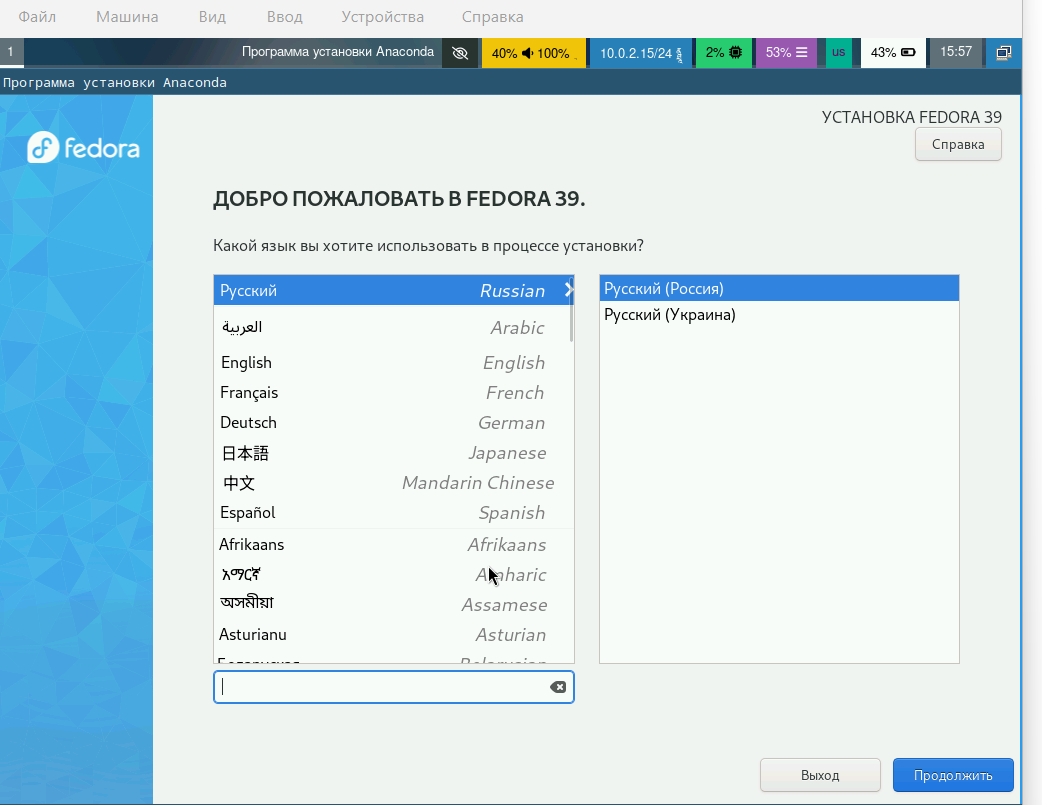
\includegraphics[width=\linewidth,height=0.66\textheight,keepaspectratio]{image/image7.png}

}

\caption{Выбор языка для ВМ}

\end{figure}%
\end{frame}

\begin{frame}{Установка Fedora Sway}
\phantomsection\label{ux443ux441ux442ux430ux43dux43eux432ux43aux430-fedora-sway-7}
Выберем диск для установки.

\begin{figure}[H]

{\centering 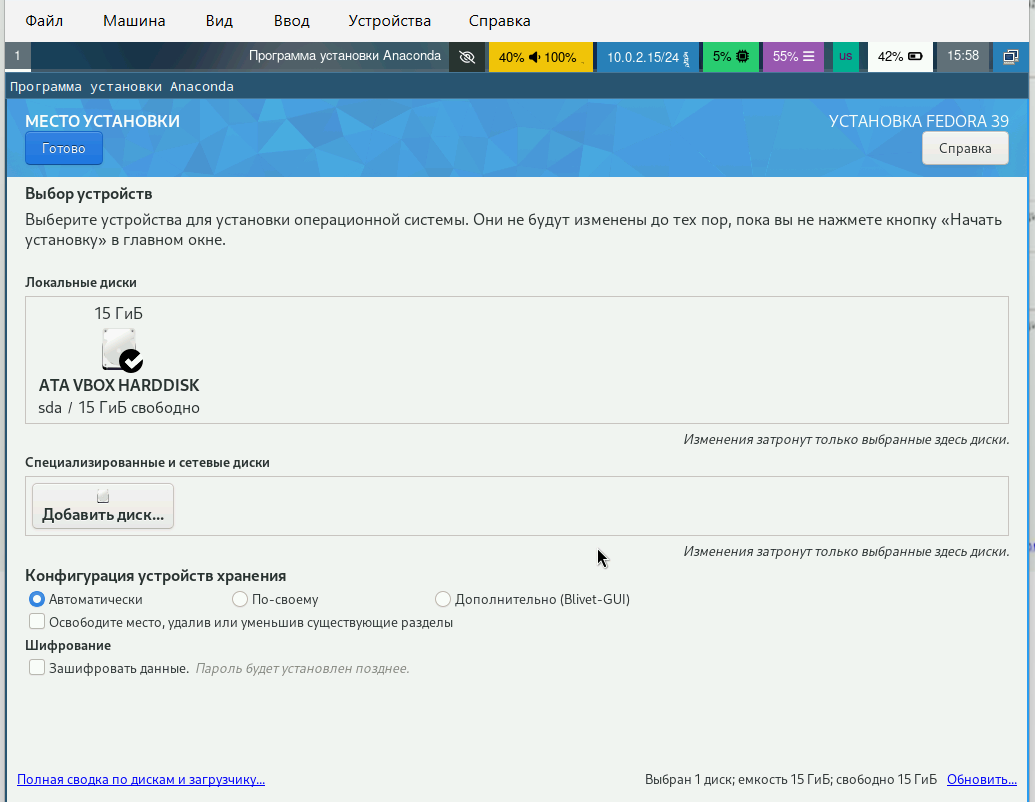
\includegraphics[width=\linewidth,height=0.66\textheight,keepaspectratio]{image/image8.png}

}

\caption{Выбор диска для установки}

\end{figure}%
\end{frame}

\begin{frame}{Установка Fedora Sway}
\phantomsection\label{ux443ux441ux442ux430ux43dux43eux432ux43aux430-fedora-sway-8}
Включим учетную запись root и укажем пароль для нее.

\begin{figure}[H]

{\centering 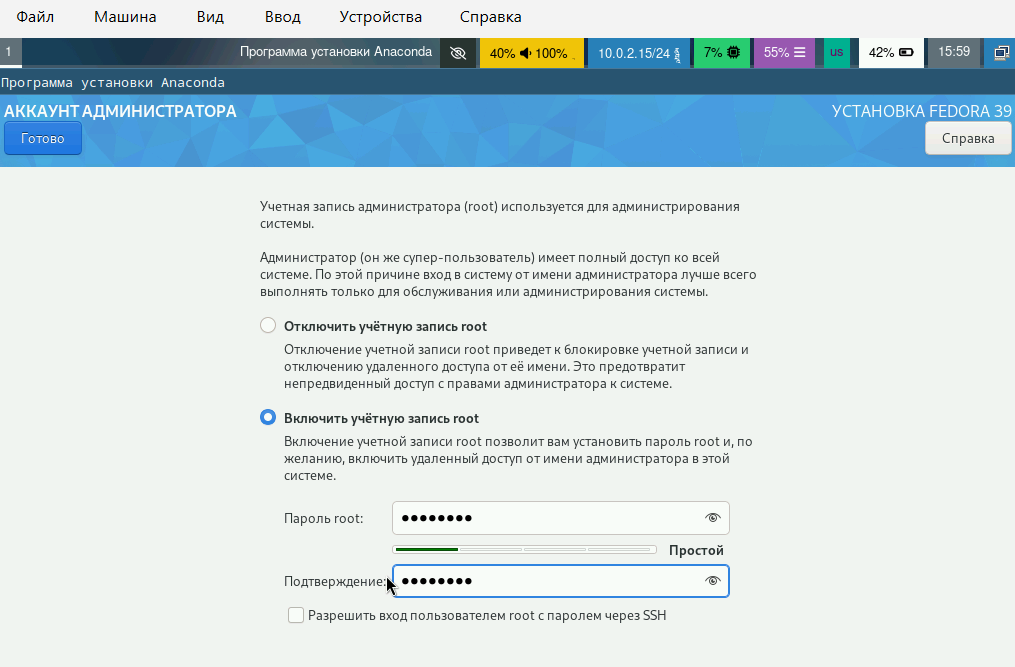
\includegraphics[width=\linewidth,height=0.66\textheight,keepaspectratio]{image/image9.png}

}

\caption{Включение учетной записи root}

\end{figure}%
\end{frame}

\begin{frame}{Установка Fedora Sway}
\phantomsection\label{ux443ux441ux442ux430ux43dux43eux432ux43aux430-fedora-sway-9}
Создадим свою учетную запись, укажем имя пользователя.

\begin{figure}[H]

{\centering 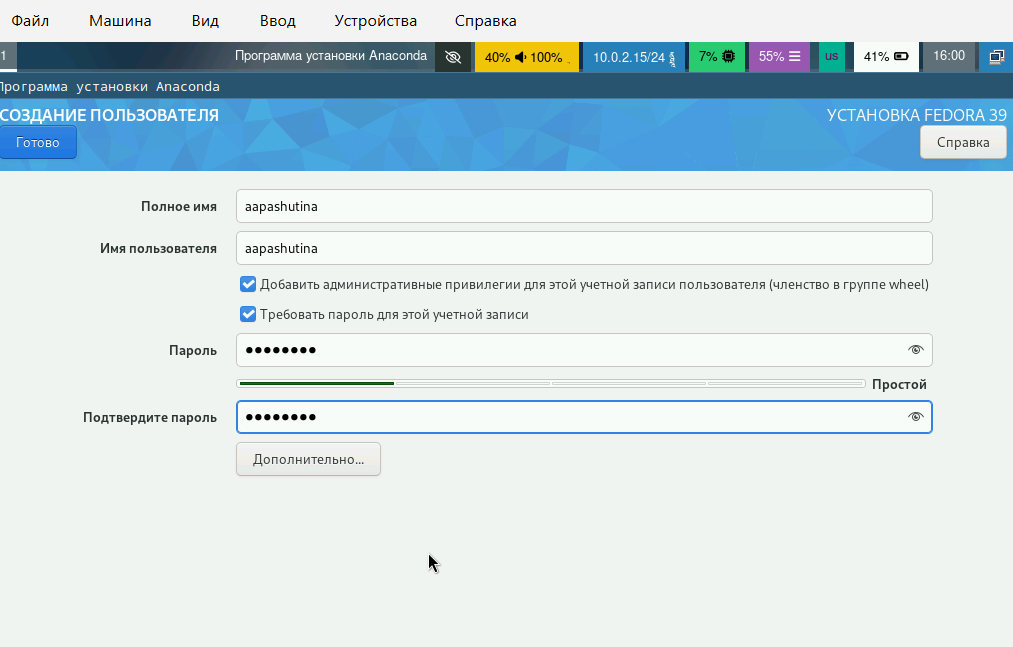
\includegraphics[width=\linewidth,height=0.66\textheight,keepaspectratio]{image/image10.png}

}

\caption{Создание учетной записи пользователя}

\end{figure}%
\end{frame}

\begin{frame}{Установка Fedora Sway}
\phantomsection\label{ux443ux441ux442ux430ux43dux43eux432ux43aux430-fedora-sway-10}
Далее начался этап загрузки, после которого мы можем изъять загрузочный
диск.

\begin{figure}[H]

{\centering 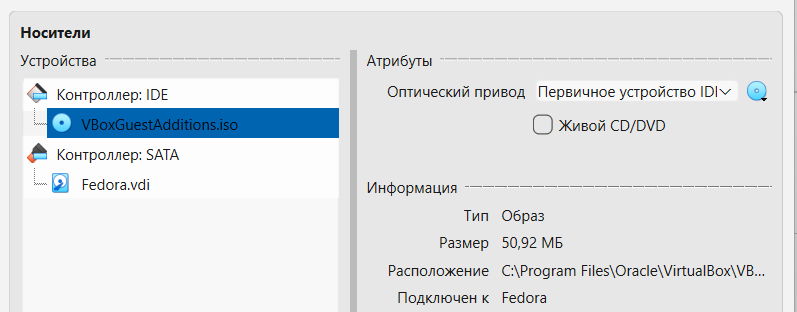
\includegraphics[width=\linewidth,height=0.66\textheight,keepaspectratio]{image/image11.png}

}

\caption{Изъятие загрузочного диска}

\end{figure}%
\end{frame}

\begin{frame}{Установка Fedora Sway}
\phantomsection\label{ux443ux441ux442ux430ux43dux43eux432ux43aux430-fedora-sway-11}
Загрузим ВМ и перейдем в режим суперпользователя с помощью команды sudo
-i.

\begin{figure}[H]

{\centering 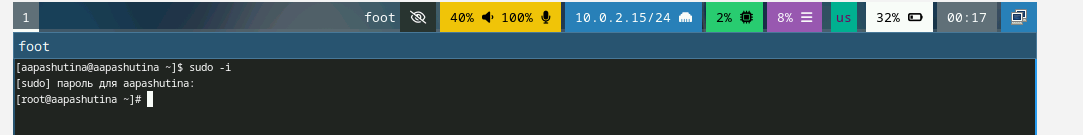
\includegraphics[width=\linewidth,height=0.66\textheight,keepaspectratio]{image/image12.png}

}

\caption{Переход в режим суперпользователя}

\end{figure}%
\end{frame}

\begin{frame}{Установка Fedora Sway}
\phantomsection\label{ux443ux441ux442ux430ux43dux43eux432ux43aux430-fedora-sway-12}
Обновим все пакеты с помощью команды dnf.

\begin{figure}[H]

{\centering 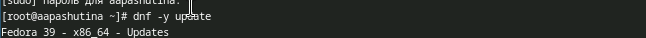
\includegraphics[width=\linewidth,height=0.66\textheight,keepaspectratio]{image/image13.png}

}

\caption{Обновление пакетов}

\end{figure}%
\end{frame}

\begin{frame}{Установка Fedora Sway}
\phantomsection\label{ux443ux441ux442ux430ux43dux43eux432ux43aux430-fedora-sway-13}
Установим mc и tmux с помощью команды dnf.

\begin{figure}[H]

{\centering 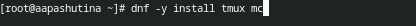
\includegraphics[width=\linewidth,height=0.66\textheight,keepaspectratio]{image/image14.png}

}

\caption{Установка tmux и mc}

\end{figure}%
\end{frame}

\begin{frame}{Установка Fedora Sway}
\phantomsection\label{ux443ux441ux442ux430ux43dux43eux432ux43aux430-fedora-sway-14}
Установим dnf-automatic.

\begin{figure}[H]

{\centering 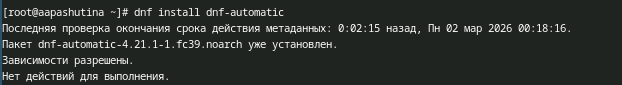
\includegraphics[width=\linewidth,height=0.66\textheight,keepaspectratio]{image/image15.png}

}

\caption{Установка dnf-automatic}

\end{figure}%
\end{frame}

\begin{frame}{Установка Fedora Sway}
\phantomsection\label{ux443ux441ux442ux430ux43dux43eux432ux43aux430-fedora-sway-15}
Включим сценарий автообновления.

\begin{figure}[H]

{\centering 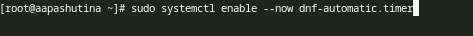
\includegraphics[width=\linewidth,height=0.66\textheight,keepaspectratio]{image/image16.png}

}

\caption{Включение сценария автообновления}

\end{figure}%
\end{frame}

\begin{frame}{Установка Fedora Sway}
\phantomsection\label{ux443ux441ux442ux430ux43dux43eux432ux43aux430-fedora-sway-16}
Выключим SELinux, отредактировав файл /etc/selinux/config следующим
образом.

\begin{figure}[H]

{\centering 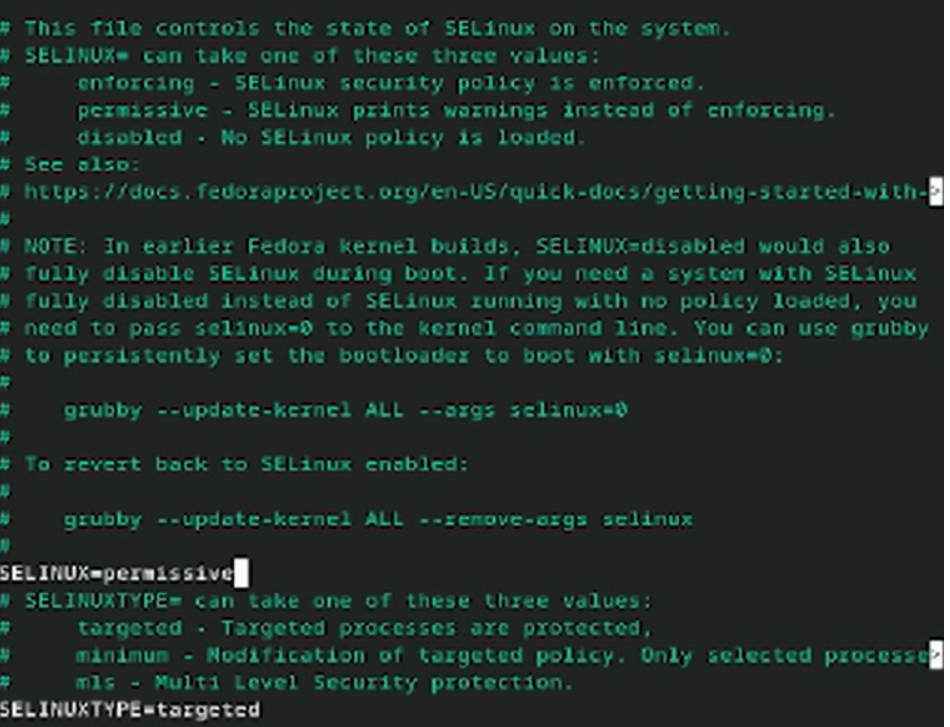
\includegraphics[width=\linewidth,height=0.66\textheight,keepaspectratio]{image/image17.png}

}

\caption{Отключение SELinux}

\end{figure}%
\end{frame}

\begin{frame}{Установка Fedora Sway}
\phantomsection\label{ux443ux441ux442ux430ux43dux43eux432ux43aux430-fedora-sway-17}
Запустим tmux.

\begin{figure}[H]

{\centering 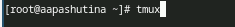
\includegraphics[width=\linewidth,height=0.66\textheight,keepaspectratio]{image/image18.png}

}

\caption{Запуск tmux}

\end{figure}%
\end{frame}

\begin{frame}{Установка Fedora Sway}
\phantomsection\label{ux443ux441ux442ux430ux43dux43eux432ux43aux430-fedora-sway-18}
Перейдем в режим root.

\begin{figure}[H]

{\centering 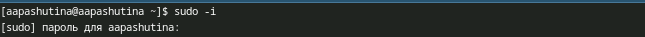
\includegraphics[width=\linewidth,height=0.66\textheight,keepaspectratio]{image/image19.png}

}

\caption{Переход в режим root}

\end{figure}%
\end{frame}

\begin{frame}{Установка Fedora Sway}
\phantomsection\label{ux443ux441ux442ux430ux43dux43eux432ux43aux430-fedora-sway-19}
Установим Development Tools.

\begin{figure}[H]

{\centering 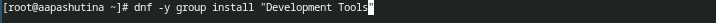
\includegraphics[width=\linewidth,height=0.66\textheight,keepaspectratio]{image/image20.png}

}

\caption{Установка Development Tools}

\end{figure}%
\end{frame}

\begin{frame}{Установка Fedora Sway}
\phantomsection\label{ux443ux441ux442ux430ux43dux43eux432ux43aux430-fedora-sway-20}
Установим dkms с помощью команды dnf.

\begin{figure}[H]

{\centering 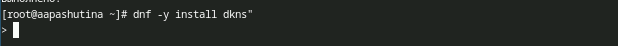
\includegraphics[width=\linewidth,height=0.66\textheight,keepaspectratio]{image/image21.png}

}

\caption{Установка dkms}

\end{figure}%
\end{frame}

\begin{frame}{Установка Fedora Sway}
\phantomsection\label{ux443ux441ux442ux430ux43dux43eux432ux43aux430-fedora-sway-21}
Подключим образ диска дополнений гостевой ОС.

\begin{figure}[H]

{\centering 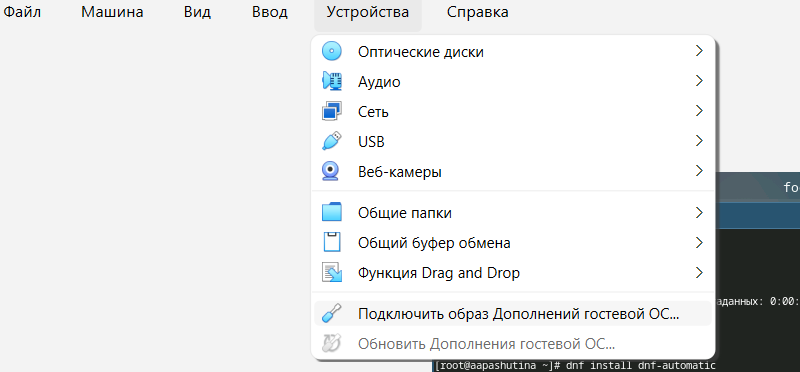
\includegraphics[width=\linewidth,height=0.66\textheight,keepaspectratio]{image/image22.png}

}

\caption{Подключение образа диска дополнений}

\end{figure}%
\end{frame}

\begin{frame}{Установка Fedora Sway}
\phantomsection\label{ux443ux441ux442ux430ux43dux43eux432ux43aux430-fedora-sway-22}
Примонтируем его и запустим скрипт-установщик.

\begin{figure}[H]

{\centering 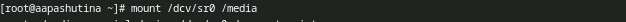
\includegraphics[width=\linewidth,height=0.66\textheight,keepaspectratio]{image/image23.png}

}

\caption{Монтирование диска и запуск установщика}

\end{figure}%
\end{frame}

\begin{frame}{Установка Fedora Sway}
\phantomsection\label{ux443ux441ux442ux430ux43dux43eux432ux43aux430-fedora-sway-23}
Создадим файл конфигурации клавиатуры.

\begin{figure}[H]

{\centering 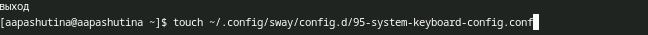
\includegraphics[width=\linewidth,height=0.66\textheight,keepaspectratio]{image/image24.png}

}

\caption{Создание файла конфигурации клавиатуры}

\end{figure}%
\end{frame}

\begin{frame}{Установка Fedora Sway}
\phantomsection\label{ux443ux441ux442ux430ux43dux43eux432ux43aux430-fedora-sway-24}
Вставим в него предложенный текст.

\begin{figure}[H]

{\centering 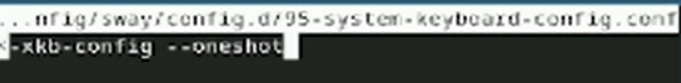
\includegraphics[width=\linewidth,height=0.66\textheight,keepaspectratio]{image/image25.png}

}

\caption{Вставка текста конфигурации}

\end{figure}%
\end{frame}

\begin{frame}{Установка Fedora Sway}
\phantomsection\label{ux443ux441ux442ux430ux43dux43eux432ux43aux430-fedora-sway-25}
Теперь поменяем настройки клавиатуры на следующие.

\begin{figure}[H]

{\centering 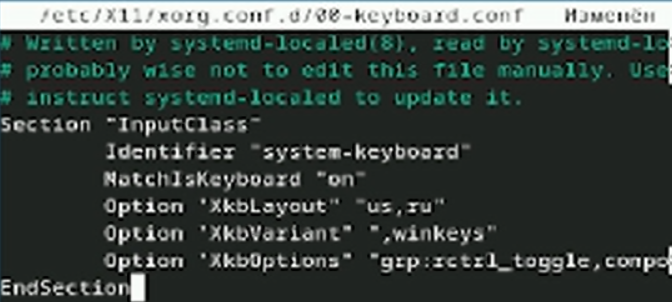
\includegraphics[width=\linewidth,height=0.66\textheight,keepaspectratio]{image/image26.png}

}

\caption{Смена настроек клавиатуры}

\end{figure}%
\end{frame}

\begin{frame}{Установка Fedora Sway}
\phantomsection\label{ux443ux441ux442ux430ux43dux43eux432ux43aux430-fedora-sway-26}
Поменяем название хоста согласно соглашению об именовании с помощью
команды hostnamectl.

\begin{figure}[H]

{\centering 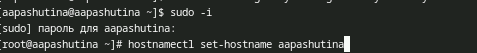
\includegraphics[width=\linewidth,height=0.66\textheight,keepaspectratio]{image/image27.png}

}

\caption{Смена названия хоста}

\end{figure}%
\end{frame}

\begin{frame}{Установка Fedora Sway}
\phantomsection\label{ux443ux441ux442ux430ux43dux43eux432ux43aux430-fedora-sway-27}
Добавим нашего пользователя в группу vboxsf.

\begin{figure}[H]

{\centering 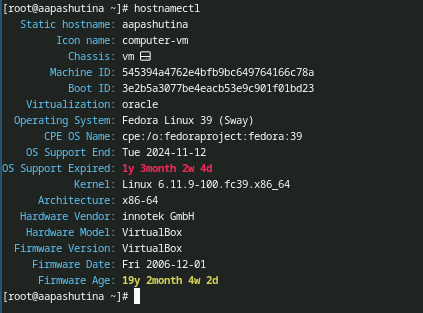
\includegraphics[width=\linewidth,height=0.66\textheight,keepaspectratio]{image/image28.png}

}

\caption{Добавление пользователя в группу vboxsf}

\end{figure}%
\end{frame}

\begin{frame}{Установка Fedora Sway}
\phantomsection\label{ux443ux441ux442ux430ux43dux43eux432ux43aux430-fedora-sway-28}
Создаем общую папку в терминале хост-машины.

\begin{figure}[H]

{\centering 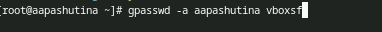
\includegraphics[width=\linewidth,height=0.66\textheight,keepaspectratio]{image/image29.png}

}

\caption{Создание общей папки}

\end{figure}%
\end{frame}

\begin{frame}{Установка Fedora Sway}
\phantomsection\label{ux443ux441ux442ux430ux43dux43eux432ux43aux430-fedora-sway-29}
Теперь установим pandoc.

\begin{figure}[H]

{\centering 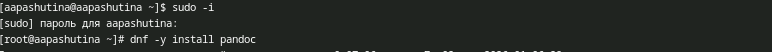
\includegraphics[width=\linewidth,height=0.66\textheight,keepaspectratio]{image/image30.png}

}

\caption{Установка pandoc}

\end{figure}%
\end{frame}

\begin{frame}{Установка Fedora Sway}
\phantomsection\label{ux443ux441ux442ux430ux43dux43eux432ux43aux430-fedora-sway-30}
Скачаем pandoc-crossref, распакуем его с помощью tar и перенесем в папку
/usr/local/bin.

\begin{figure}[H]

{\centering 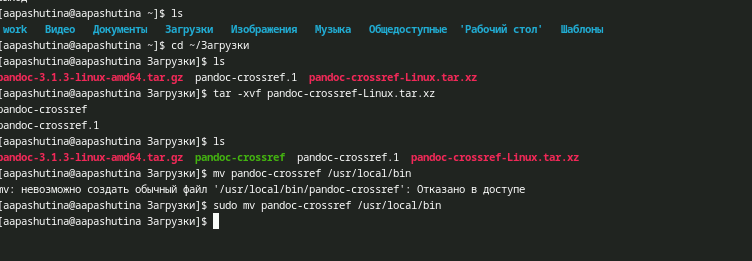
\includegraphics[width=\linewidth,height=0.66\textheight,keepaspectratio]{image/image31.png}

}

\caption{Установка pandoc-crossref}

\end{figure}%
\end{frame}

\begin{frame}{Установка Fedora Sway}
\phantomsection\label{ux443ux441ux442ux430ux43dux43eux432ux43aux430-fedora-sway-31}
Установим texlive.

\begin{figure}[H]

{\centering 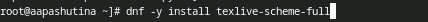
\includegraphics[width=\linewidth,height=0.66\textheight,keepaspectratio]{image/image32.png}

}

\caption{Установка texlive}

\end{figure}%
\end{frame}

\section{Домашнее
задание}\label{ux434ux43eux43cux430ux448ux43dux435ux435-ux437ux430ux434ux430ux43dux438ux435}

\begin{frame}{Домашнее задание}
\phantomsection\label{ux434ux43eux43cux430ux448ux43dux435ux435-ux437ux430ux434ux430ux43dux438ux435-1}
\begin{columns}[c]
\begin{column}{0.6\linewidth}
С помощью dmesg получим следующую информацию:

\begin{itemize}[<+->]
\tightlist
\item
  Версия ядра Linux (Linux version) --- 6.11.9
\item
  Частота процессора (Detected Mhz processor) --- 2611.210
\item
  Модель процессора (CPU0) --- Core i5-13420H
\item
  Объём доступной оперативной памяти (Memory available) --- 8071424K
\item
  Тип обнаруженного гипервизора (Hypervisor detected) --- KVM
\end{itemize}
\end{column}

\begin{column}{0.3\linewidth}
\begin{figure}[H]

{\centering 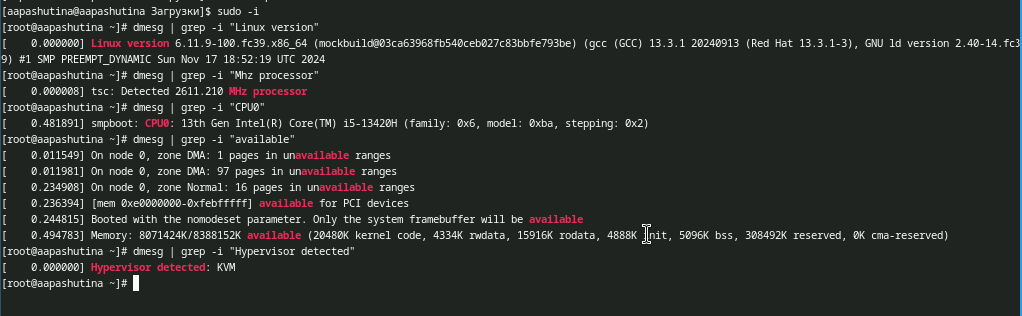
\includegraphics[width=\linewidth,height=0.66\textheight,keepaspectratio]{image/image33.png}

}

\caption{Информация из dmesg}

\end{figure}%
\end{column}
\end{columns}
\end{frame}

\begin{frame}{Домашнее задание}
\phantomsection\label{ux434ux43eux43cux430ux448ux43dux435ux435-ux437ux430ux434ux430ux43dux438ux435-2}
\begin{itemize}[<+->]
\tightlist
\item
  Тип файловой системы корневого раздела --- BTRFS
\item
  Последовательность монтирования файловых систем --- EXT4-fs
\end{itemize}

\begin{figure}[H]

{\centering 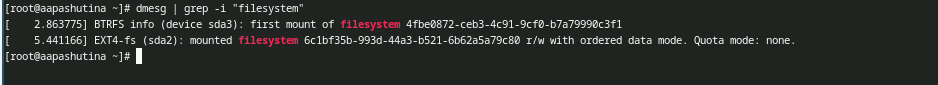
\includegraphics[width=\linewidth,height=0.8\textheight,keepaspectratio]{image/image34.png}

}

\caption{Информация о файловой системе}

\end{figure}%
\end{frame}

\section{Выводы}\label{ux432ux44bux432ux43eux434ux44b}

\begin{frame}{Выводы}
\phantomsection\label{ux432ux44bux432ux43eux434ux44b-1}
Были получены навыки работы в системе Fedora Sway: проведена установка
системы, установлены необходимые для последующей работы пакеты и
произведена базовая настройка системы.
\end{frame}




\end{document}
